
%(BEGIN_QUESTION)
% Copyright 2007, Tony R. Kuphaldt, released under the Creative Commons Attribution License (v 1.0)
% This means you may do almost anything with this work of mine, so long as you give me proper credit

Calculate the height of glycerine ($\gamma$ = 78.6 lb/ft$^{3}$) in a vertical tube if there is 21 PSI of hydrostatic pressure at the bottom of the tube:

$$\includegraphics[width=15.5cm]{i02951x01.eps}$$

Glycerine height = \underbar{\hskip 50pt} ft

\vskip 30pt

Also, calculate the height of castor oil ($\gamma$ = 60.5 lb/ft$^{3}$) necessary to generate the exact same amount of pressure:

\vskip 10pt

Castor oil height = \underbar{\hskip 50pt} ft

\underbar{file i02951}
%(END_QUESTION)





%(BEGIN_ANSWER)

Glycerine height = \underbar{\bf 38.46} ft

\vskip 10pt

Castor oil height = \underbar{\bf 49.96} ft

%(END_ANSWER)





%(BEGIN_NOTES)

%INDEX% Physics, static fluids: hydrostatic pressure

%(END_NOTES)


